\documentclass[%
 aip,
% jmp,
% bmf,
% sd,
% rsi,
cp,  % Conference Proceedings
 amsmath,amssymb,%nobibnotes,
% preprint,%
 reprint,%
%author-year,%
%author-numerical,%
]{revtex4-2}

\usepackage{graphicx}% Include figure files
\usepackage{dcolumn}% Align table columns on decimal point
\usepackage{bm}% bold math
%\usepackage[mathlines]{lineno}% Enable numbering of text and display math
%\linenumbers\relax % Commence numbering lines

\usepackage[utf8]{inputenc}
\usepackage[T1]{fontenc}
%% Loads a Times-like font. You can also load
%% {newtxtext,newtxtmath}, but not {times}, 
%% {txfonts} nor {mathtpm} as these packages
%% are obsolete and have been known to cause problems.
\usepackage{mathptmx} 
\bibliographystyle{apsrev4-2}

\begin{document}

\title{Comparative Analysis of Different Hashing Algorithms for Data Deduplication}% Force line breaks with \\

\author{Kuldeep Vayadande} % Write as First name Surname
 \email{kuldeep.vayadande@gmail.com}
\author{Arunav Chandra}%
 \email{arunav.chandra20@vit.edu}
 \author{Anveshika Kamble}%
 \email{anveshika.kamble20@vit.edu}
 \author{Rohit Arole}%
 \email{rohit.arole20@vit.edu}
 \author{Sukhpreet Singh Bhatti}%
 \email{sukhpreet.bhatti20@vit.edu}
 \author{Bijin Jiby}%
 \email{bijin.jiby20@vit.edu}
\affiliation{
  Department of Information Technology, Vishwakarma Institute of Technology, Pune, India% Force line breaks with \\ if necessary
}

\date{\today} % It is always \today, today, but any date may be explicitly specified
              % Not printed for conference proceedings

\begin{abstract}
Hashing is an essential application involved primarily in ensuring a strong and secure application. The massive amount of data produced these days are coming from various online sources, and all types of data need to be stored for using it in future. But this data has lots of duplication, which makes the storage of those files slow and increases the redundancy in the backups. So, to improve the efficiency of these applications, data deduplication is used, which means storing the unique data along with where it has been used.%
We have used different hashing algorithms such as SHA1, MD5, SHA256 and done a comparative analysis of all the algorithms. Our results show that as the algorithms have progressed, their performance has increased significantly, in terms of data deduplication as well as encryption. This is because of the internal working of the algorithms, as MD5 reruns the whole process multiple times, but as we compare the SHA256 algorithm, the data is simply passed under a mathematical function, which converts the plaintext into hashed text.
\end{abstract}

\maketitle

\section{\label{sec:introduction}INTRODUCTION}

With increasing data these days, it has become very tough to store and use data. Along with the data being produced by small enterprises, the majority of the data being produced is from machines, social media, and cookies being collected by various websites for improving the user experience. The data being collected by machines is of various types again, such as system logs, wearable device data, and data collected by various IOT sensors. This type of data grows exponentially along with time, as it keeps recurring and written separately over the older files. This data is mixed with the data collected by user applications, websites and cloud programs that involve the use of the data. 

Social media providers also produce data in abundance. If we elaborate on it with an example, it would be a comment on any post, along with the threads of comments on the post. If each comment on the post has another thread of comments following it, the number of comments grows exponentially again. This data requires more storage if it is being employed for any business application, where the data of the customer, his/her likes, dislikes, and engagement are being collected again to improve their experience along with providing them with better sales-related options. This data can further be expanded to similar types of users, and thus a massive web of data is created. This also has a collection of demographics; behavioural data of users being captured. 

The third type of data is transactional data. It collects various quantifiable information from each transaction such as orders, invoices, storage records, and demographics. This data is further employed to increase the sales of various products by deploying various machine learning algorithms such as market basket analysis, recommendation engines etc. This helps boost the sales of the products and businesses.

\section{\label{sec:litreview}Literature Survey}
The authors \cite{mb15} talk about various ways in which data can be deduplicated while casting a shadow on what data deduplication is and its importance in today’s time. They have split the process of data deduplication into a pipeline, where after undergoing all the processes, the final data is deduplicated. We have used this pipeline in our project as the base structure for deduplicating our files, i.e., creating chunks, and metadata of each chunk, then processing them. These chunks are then scanned for finding duplicates among them. The authors propose to employ their data deduplication methods on images and videos in the future, while also parallelizing the deduplication process to improve the performance of the algorithm while giving a faster result.

The authors \cite{hlz10} talk about different data deduplication techniques, which include multiple data deduplication strategies such as file-level, and block level data deduplication. They have explained about different uses of various hashing functions such as MD5 and SHA1 for hashing the data for deduplication. They have even tried the implementation for byte-sized data. We have referenced this paper as our base paper to focus on block-sized data to compare the performance of various cryptographic functions on data deduplication.

The Authors \cite{ma14} talk about variable size data deduplication and how it is better than other strategies with the help of creating a hash for each chunk. This technique enables us to have better storage efficiency which directly improves efficiency by allowing storage to transfer and handle large amounts of data. Multiple storage optimization techniques are also elaborated upon along with chunk-based data deduplication techniques and their implementations.

The authors \cite{cb18} perform a comparative study on various data deduplication techniques like File level chunking, block level chunking, and deduplication with respect to location (source and target side), and with respect to time. They also identified the sources of redundancy in big data workloads and discussed possible solutions. Security and Data privacy is still relatively unexplored domain in Data deduplication and the authors emphasize the immediate need for work to be done for the concept to be used on a normalized basis. 

Authors \cite{xjfdshfzz16} have tried to summarize the work done in data deduplication technologies with parts discussing future scopes and open problems in the field, authors have also tried to cover the basic flow of performing data deduplication by going in deep into each part like chunking, indexing, hashing, compression, and management. authors have also explained the state-of-the-art methods used for chunking and hashing and performed comparative analysis on the following as well and went deep not just solving that part but have also explained and stated different ways in which the process can be accelerated like GPU or multicore approach, and finally talking about data restoration and garbage collection.

Authors \cite{ls} have talked about using SHA-256 to detect duplicate data and provided solution to remove it. authors of the papers had used two methods aliasing and data encoding  for finding data deduplicates and exact copies, authors have also did a detailed comparison of data deduplication techniques of different product companies, they had used SHA 256 instead of traditional SHA-1 , MD5 because they fail to produce required accuracy in big and huge data, after implementing SHA 256 and SHA-512 based on 62 bit architecture they have compared the space and time complexity of used algorithms. As data has been increasing tremendously due to the increase in global usage of internet services. There have been many problems in data cloud handling. Big data is a major concern in cloud computing. 
Shengmei Luo and other authors \cite{lzwkl15} of the paper have discussed data deduplication in the cloud computing domain. They have discussed various techniques that have been employed in cloud storage utilities for making the cost of data storage in cloud-based services less expensive by introducing the concept of distributed data deduplication. They named their system Boaft. Boaft uses multiple servers for storing the references of data. It has a very efficient routing algorithm for identifying the location of the data in the respective server which makes it a system with a very high deduplication ratio.

In this paper \cite{mkbckk12} the potential for data deduplication at HPC centres, which are among the most demanding storage providers, is the subject of the first research presented. This potential for capacity decreases for 4 data centres has been objectively examined (BSC, DKRZ, RENCI, RWTH). They have examined over one PB (1212 TB) of live file system data, in contrast to earlier deduplication research that mostly focused on backup data. The analysis demonstrates that data deduplication techniques may often eliminate 20\% to 30\% of this internet data, with certain data sets reaching up to 70\%. Only a subfile deduplication strategy can accomplish this decrease, while whole-file comparison strategies only provide marginal capacity reductions.

In this paper \cite{ylstg21}, an effective large data deduplication strategy that protects privacy is suggested in the study for a two-level multi-domain architecture. Specifically, their technique preserves data confidentiality under multi-domain deduplication and thwarts brute-force assaults by producing a random tag and a fixed number of random ciphertexts for each datum. the system can effectively safeguard the message equality information from disclosure by limiting the intra- and inter-deduplication operations to the agent and cloud service provider, respectively. A thorough security study demonstrates that our plan successfully accomplishes privacy preservation for both data integrity and message equality information while fending off brute-force assaults. Additionally, thorough simulations show that our strategy greatly outperforms the other available rival strategies, particularly in terms of computing cost and the temporal complexity of the duplication search.

The authors have \cite{kp} have discussed the increase in demand for data deduplication. They have well explained the benefits of data deduplication. Due to the rising data, it needs tons of storage utilities which are difficult to maintain. Data deduplication is one of the techniques in data management for compressing data to reduce storage problems. They store the references of the file encrypted with differential privilege keys. To make this system more secure and restricted to unauthorized users. They have introduced here a new advanced feature of data deduplication such that the user having a specific access request can only perform the actions associated with that privilege key. This feature makes the owner and user-side data secure and easier to access. The paper here proposed a design of authorized data deduplication. Traditional data deduplication services only include the storing of data in one place and providing a reference but as it advances the new system has deduplication with auditing the user`s access permissions.

\section{\label{sec:methodology}METHODOLOGY}

\subsubsection{\label{sec:steps}Steps Involved }
\begin{enumerate}
\item {File Extraction: 
The entire contents of the files are read and stored into an array while keeping in check for empty lines and writing them into a new text file for future reference.}
\item{Binary Conversion: 
The contents of the array are converted into binary format to prepare them for proper pipelining within the hashing algorithms.}
\item{MD5 Algorithm: 
We apply MD5 hashing algorithm on the binary text by passing each binary file under a loop.}
\item{Storing and deduplication: 
We then store each data into a hash table to check if the data exists else if the data exits then the index of the file is appended to the list of the hash table value.}
\item{Final List returned: 
We get the final list with all the unique values available and their indexes along with them.}
\end{enumerate}

As illustrated in Fig.\ref{fig:MD5}, we can understand the various processes involved in data deduplication using a particular hashing algorithm, e.g., MD5. We have used many more algorithms such as SHA1, SHA256, etc. to compare and analyze which type of algorithm works best for our task, i.e., data deduplication.

\subsubsection{\label{sec:algos}Algorithms }
We have used three different types of hashing algorithms in our model, MD5, SHA1, and SHA256. 
\begin{enumerate}
    \item {MD5 Algorithm}
    MD5 algorithm is also called as Message Digest algorithm, which takes input data and applies a series of message digest functions to it to hash the data. This can be seen in Fig.\ref{fig:MD5}%
    \begin{figure}
\includegraphics{Picture12.eps}% Here is how to import EPS art
\caption{ Process Flow Chart of MD5 Algorithm.}
\label{fig:MD5}
\end{figure}
    \begin{itemize}
        \item {Split data into blocks}
        \item{add padding bits (0) to the blocks to convert them into a length of 64 bits less than a multiple of 512. }
        \item{To the previously created padded value, we add the length bit, i.e., 64 bits as length of the data. }
        \item{Apply a series of four transitions on the blocks}
        \item{Combine all the blocks to create a final hash value.}
        \item{Return the hashed value of the original data.}
    \end{itemize}

    \begin{figure}
\includegraphics{Picture2.eps}% Here is how to import EPS art
\caption{SHA1 Algorithm }
\label{fig:sha1}
\end{figure}%
    \item{SHA1 Algorithm}
    This algorithm is also called as Secure Hash Algorithm 1. It takes input and returns a 160-bit hashed value as output. 
    \begin{itemize}
        \item{Split data into blocks.}
        \item{Add padding bits (0) to the blocks to convert them into a length of 64 bits less than a multiple of 512. }
        \item{To the previously created padded value, we add the length bit, i.e., 64 bits as length of the data.}
        \item{Create a hash state buffer, that is an array of 5 32-bit integers in a hexadecimal format. }
        \item{We divide the 512 blocks into 16 blocks of 32-bit size.}
        \item{The 16 blocks are converted to 80 blocks by applying a hash function on the current block, and returning the hashed value as the next value, until all 80 values have been created.}
        \item{The 80 bits created are compressed into the final 160-bit hashed value output.}
        \item{The hashed value is returned as the final output.}
    \end{itemize}
\end{enumerate}%

\section{\label{sec:results}RESULTS}
We notice that we get the best results when we use SHA256 as our hashing algorithm from Fig. \ref{fig:execTime}.
\begin{figure}
\includegraphics{Picture3.eps}% Here is how to import EPS art
\caption{Execution time of each Hashing Algorithm}
\label{fig:execTime}
\end{figure}%
We observe that for a file with around 4 lakh characters, SHA256 algorithm works the fastest in deduplicating the data, while successfully reducing the data, significantly. %

The percentage of data deduplicated  by each algorithm is same, where the data is created into separate hashes, but since the base data is same, the deduplicated percentage remains the same among all, only the time changes Fig.\ref{fig:execTime}.
\begin{figure}
    \centering
    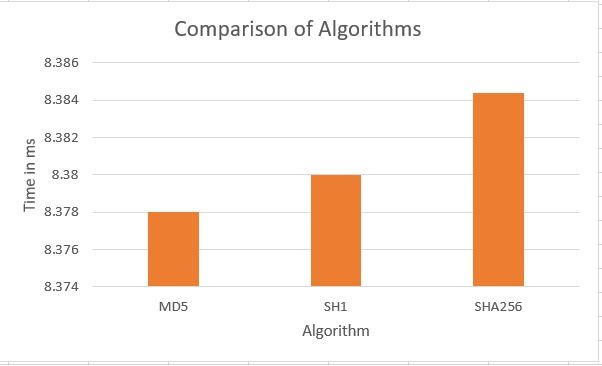
\includegraphics{time.eps}
    \caption{Comparison of Time taken to deduplicate data }
    \label{fig:my_label}
\end{figure}

\section{Conclusion}

By concluding our results and observations, we can infer that data deduplication is an essential task in today’s generation where the data present exists in petabytes and exabytes. Furthermore, we got insights into various cryptographic algorithms, which not only ensure the security of data being transferred but also helps ease the process of data deduplication.

\begin{acknowledgments}
We wish to acknowledge the support of Veritas primarily in selecting us for this sponsored project, while continuously offering us suggestions and encouragement, testing new versions, We would furthermore like to thank our faculties, and Vishwakarma Institute of Technology of Pune for giving us the opposrutnity to work on this project.
\dots.
\end{acknowledgments}

\nocite{*}
\bibliography{aipsamp}% Produces the bibliography via BibTeX.

\end{document}
%
% ****** End of file aipsamp.tex ******
